\documentclass{article}
\usepackage[utf8]{inputenc}
\usepackage{geometry}
\usepackage{enumitem}
\usepackage{hyperref}
\usepackage{xcolor}
\usepackage{graphicx}
\usepackage{array}
\usepackage{multirow}
\usepackage{amsmath, amssymb}
\usepackage{chemfig}
\usepackage{mhchem}
\usepackage{tikz}
\usepackage{setspace}
\usepackage{soul}
\usepackage{mathtools}
\usepackage{booktabs}
\usepackage{chemformula}
\usepackage{siunitx}
\usetikzlibrary{positioning, shapes, arrows.meta, decorations.pathreplacing, fit, backgrounds}
\usepackage{longtable}
\geometry{margin=1in}
\setlength{\parskip}{0.5em}
\usepackage{cancel}

\begin{document}

\begin{center}
    {\LARGE \textbf{SI Session Planning Form}}
\end{center}

\vspace{0.5cm}

\noindent
\begin{flushleft}
\textbf{SI Leader:} Brandon Cobb \\
\textbf{Session Week:} 2 \\
\textbf{Session \#:} 2 \\
\textbf{Instructor:} Professor Tramontozzi \\
\textbf{Old Plans:} \href{https://macombedu.sharepoint.com/:b:/s/ASC-SupplementalInstructionEmbeddedTutoring/EeSYqCwT_KhMolgJvXbVEjgBOyF_DevvS8BgCm1zPkQQJg?e=QJTt4o}{SharePoint} \\
\textbf{Session Goal:} Students will be able to perform measurements using measurment devices with fixed uncertainty values, record data with units, convert between units and write scienticific notation. Students are given a reference sheet for conversion factors.
\end{flushleft}

\vspace{1em}
\section*{\underline{Opener}}
{\centering\large\textbf{\hl{Take Attendance}}\par}\vspace{-0.25\baselineskip}
\noindent
\begin{tabular}{|p{4.2cm}|p{9.8cm}|}
\hline
\textbf{Collaborative Learning Techniques} & Clusters \\
\hline
\textbf{Learning Strategy} & Send a Problem \\
\hline
\textbf{Time} & 12:00---12:10 \\
\hline
\textbf{Materials} & A ruler, a scale and a shot glass. Objects including a vial (with water), a heavy fidget toy and a long fidget toy.  \\
\hline
\textbf{Lecture/Textbook/Old Plans/Slide References} & Class roster, Chapter 2: Measurments \\
\hline
\end{tabular}
\\
\vspace{0.5cm}
{\large \textbf{Definitions}}
\\
\begin{tabular}{|p{0.9\linewidth}|}
\hline
\begin{minipage}[t]{0.9\linewidth}
\begin{enumerate}
    \item \textbf{Clusters:} In Clusters, group participants are divided into smaller groups for discussion. They may also be allowed to self-select the small group they want to be in. After discussing the assigned topic, the cluster may report their findings to the large group.
    \item \textbf{Send a Problem:} Generate a list of problems. Assign a different problem to each student. Give the students a minute to complete the first step of their assigned problem. After the minute, students pass their problem to the students to their right, who then complete the second step of the problem. Continue passing the problem until the steps are completed. After, have the students present their originally-assigned problems with the completed solutions to the entire group.
\end{enumerate}
\end{minipage}
\\ \hline
\end{tabular}
\newpage
\noindent
{\large \textbf{Instructions (please provide a \hl{DETAILED} activity breakdown below (and/or attached}} \\

\begin{tabular}{|p{0.9\linewidth}|}
\hline

\vspace{0.2cm}
\begin{enumerate}
    \item The leader will pair up partners based on proximity seating. If someone is without a partner, be their partner.
    \item Each pair is given an object and are asked to measure either its mass, length or volume (respective to its object (long=length, heavy=mass, liquid=volume).
    \item Given two minutes, they will decide which measurment tool they will use and the leader will provide it to them.
    \item They are asked to measure the quantity, save the value, and forward the object and measurement device to the next pair.
    \item The next pair will measure the quantity. If one of the pairs chose the wrong tool, switch out the tool for the next pair.
    \item By turn, each group will describe their object and their measurment and measurement device.
    \item We will point out which tools are ineffective for different measurements
\end{enumerate} \\[0.5em]
Students in pairs will measure the metric for their object, then they will pass the object to a partner group and they will estimate the measurement. \\
\hline
\end{tabular}
\newpage

\noindent
{\large \textbf{Content (fully worked out problems \& answers)}} \\[0.2em]

\begin{tabular}{|p{0.9\linewidth}|}
\hline
\vspace{0.2cm}

\textbf{(1)} Convert 125 miles into kilometers. (Use $1~\text{mile} = 1.609~\text{km}$) \\
\hline
\textbf{Solution:} \\
\[
\frac{125~\cancel{\text{mi}}}{1} \times \frac{1.609~\text{km}}{1~\cancel{\text{mi}}}
= 201~\text{km}
\] \\
\hline
\end{tabular}
\newpage

\noindent
{\large \textbf{Content (fully worked out problems \& answers) continued}} \\[0.2em]
\begin{tabular}{|p{0.9\linewidth}|}
\hline
\vspace{0.2cm}

\textbf{(2)} A car travels 95.0 kilometers in 1.20 hours. What is its speed in meters per second? \\
\hline
\textbf{Solution:} \\
\[
\frac{95.0~\cancel{\text{km}}}{1} \times \frac{1000~\text{m}}{1~\cancel{\text{km}}} 
= 9.50 \times 10^4~\text{m}
\]
\[
\frac{1.20~\cancel{\text{h}}}{1} \times \frac{3600~\text{s}}{1~\cancel{\text{h}}} 
= 4320~\text{s}
\]
\[
\text{Speed} = \frac{Distance}{Time}
= \frac{9.50 \times 10^4~\text{m}}{4320~\text{s}} 
= 22.0~\text{m/s}
\] \\
\hline
\end{tabular}
\newpage

\noindent
{\large \textbf{Content (fully worked out problems \& answers) continued}} \\[0.2em]
\begin{tabular}{|p{0.9\linewidth}|}
\hline
\vspace{0.2cm}

\textbf{(3)} The density of aluminum is $2.70~\text{g/cm}^3$. What is the mass of a block of aluminum with a volume of $15.0~\text{cm}^3$? \\
\hline
\textbf{Solution:} \\
\[
\text{Density} = \frac{\text{Mass}}{\text{Volume}} \quad \Rightarrow \quad \text{Mass} = \text{Density} \times \text{Volume}
= \frac{2.70~\text{g}}{1~\cancel{\text{cm}^3}} \times \frac{15.0~\cancel{\text{cm}^3}}{1} 
= 40.5~\text{g}
\] \\
\hline
\end{tabular}
\newpage

\noindent
{\large \textbf{Content (fully worked out problems \& answers) continued}} \\[0.2em]
\begin{tabular}{|p{0.9\linewidth}|}
\hline
\vspace{0.2cm}

\textbf{(4)} A patient’s mass is 154 lb. Convert this to kilograms. (Use $1~\text{lb} = 453.6~\text{g}$) \\
\hline
\textbf{Solution:} \\
\[
\text{Mass} = \frac{154~\cancel{\text{lb}}}{1} \times \frac{453.6~\text{g}}{1~\cancel{\text{lb}}} \times \frac{1~\text{kg}}{1000~\cancel{\text{g}}}
= 69.9~\text{kg}
\] \\
\hline
\end{tabular}
\newpage

\noindent
{\large \textbf{Content (fully worked out problems \& answers) continued}} \\[0.2em]
\begin{tabular}{|p{0.9\linewidth}|}
\hline
\vspace{0.2cm}

\textbf{(5)} Convert 0.750 L into cubic centimeters. (Use $1~\text{L} = 1000~\text{cm}^3$) \\
\hline
\textbf{Solution:} \\
\[
\text{Volume} = \frac{0.750~\cancel{\text{L}}}{1} \times \frac{1000~\text{cm}^3}{1~\cancel{\text{L}}} 
= 750~\text{cm}^3
\] \\
\hline
\end{tabular}
\newpage

\noindent
{\large \textbf{Content (fully worked out problems \& answers) continued}} \\[0.2em]
\begin{tabular}{|p{0.9\linewidth}|}
\hline
\vspace{0.2cm}

\textbf{(6)} A cube has an edge length of 2.50 cm. What is its volume in cubic meters? \\
\hline
\textbf{Solution:} \\
\[
\left(\frac{2.50~\text{cm}}{1}\right)^3 = \frac{15.625~\text{cm}^3}{1}
\]
\[
\text{Volume} = \frac{15.625~\cancel{\text{cm}^3}}{1} \times \frac{1~\text{m}}{100~\cancel{\text{cm}}} \times \frac{1~\text{m}}{100~\cancel{\text{cm}}} \times \frac{1~\text{m}}{100~\cancel{\text{cm}}}
= 1.56 \times 10^{-5}~\text{m}^3
\] \\
\hline
\end{tabular}
\newpage

\noindent
{\large \textbf{Content (fully worked out problems \& answers) continued}} \\[0.2em]
\begin{tabular}{|p{0.9\linewidth}|}
\hline
\vspace{0.2cm}

\textbf{(7)} The density of mercury is $13.6~\text{g/mL}$. What is the volume (in mL) of a 125 g sample of mercury? \\
\hline
\textbf{Solution:} \\
\[
\text{Density} = \frac{\text{Mass}}{\text{Volume}} \quad \Rightarrow \quad \text{Volume} = \frac{\text{Mass}}{\text{Density}}
= \frac{125~\text{g}}{1} \times \frac{1~\cancel{\text{mL}}}{13.6~\cancel{\text{g}}} 
= 9.19~\text{mL}
\] \\
\hline
\end{tabular}
\newpage
\noindent
{\large \textbf{Content (fully worked out problems \& answers) continued}} \\[0.2em]
\begin{tabular}{|p{0.9\linewidth}|}
\hline
\vspace{0.2cm}

\textbf{(8)} Convert 3.25 hours to seconds. \\
\hline
\textbf{Solution:} \\
\[
\text{Time} = \frac{3.25~\cancel{\text{h}}}{1} \times \frac{60~\cancel{\text{min}}}{1~\cancel{\text{h}}} \times \frac{60~\text{s}}{1~\cancel{\text{min}}}
= 1.17 \times 10^4~\text{s}
\] \\
\hline
\end{tabular}
\newpage

\noindent
{\large \textbf{Content (fully worked out problems \& answers) continued}} \\[0.2em]
\begin{tabular}{|p{0.9\linewidth}|}
\hline
\vspace{0.2cm}

\textbf{(9)} Convert 48.0 inches to centimeters. (Use $1~\text{in} = 2.54~\text{cm}$) \\
\hline
\textbf{Solution:} \\
\[
\text{Distance} = \frac{48.0~\cancel{\text{in}}}{1} \times \frac{2.54~\text{cm}}{1~\cancel{\text{in}}}
= 122~\text{cm}
\] \\
\hline
\end{tabular}
\newpage

\noindent
{\large \textbf{Content (fully worked out problems \& answers) continued}} \\[0.2em]
\begin{tabular}{|p{0.9\linewidth}|}
\hline
\vspace{0.2cm}

\textbf{(10)} Convert 2.50 gallons to liters. (Use $1~\text{gal} = 3.785~\text{L}$) \\
\hline
\textbf{Solution:} \\
\[
\text{Volume} = \frac{2.50~\cancel{\text{gal}}}{1} \times \frac{3.785~\text{L}}{1~\cancel{\text{gal}}}
= 9.46~\text{L}
\] \\
\hline
\end{tabular}
\newpage

\noindent
{\large \textbf{Content (fully worked out problems \& answers) continued}} \\[0.2em]
\begin{tabular}{|p{0.9\linewidth}|}
\hline
\vspace{0.2cm}

\textbf{(11)} A metal sample has mass $12.3~\text{g}$ and density $8.90~\text{g/cm}^3$. What is its volume in mL? \\
\hline
\textbf{Solution:} \\
\[
\frac{12.3~\text{g}}{1} \times \frac{1~\cancel{\text{cm}^3}}{8.90~\cancel{\text{g}}}
= \frac{1.38~\text{cm}^3}{1}
\]
\[
\text{Volume} = \frac{1.38~\cancel{\text{cm}^3}}{1} \times \frac{1~\text{mL}}{1~\cancel{\text{cm}^3}}
= 1.38~\text{mL}
\] \\
\hline
\end{tabular}
\newpage

\noindent
{\large \textbf{Content (fully worked out problems \& answers) continued}} \\[0.2em]
\begin{tabular}{|p{0.9\linewidth}|}
\hline
\vspace{0.2cm}

\textbf{(12)} Convert $7.50~\text{m/s}$ to $\text{km/h}$. \\
\hline
\textbf{Solution:} \\
\[
\text{Speed} = \frac{7.50~\text{m}}{1~\text{s}} \times \frac{1~\cancel{\text{km}}}{1000~\cancel{\text{m}}} \times \frac{3600~\cancel{\text{s}}}{1~\text{h}}
= 27.0~\text{km/h}
\] \\
\hline
\end{tabular}
\newpage

\noindent
{\large \textbf{Content (fully worked out problems \& answers) continued}} \\[0.2em]
\begin{tabular}{|p{0.9\linewidth}|}
\hline
\vspace{0.2cm}

\textbf{(13)} Convert $2.000~\text{ft}^2$ to $\text{m}^2$. (Use $1~\text{ft}=0.3048~\text{m}$) \\
\hline
\textbf{Solution:} \\
\[
\text{Area} = \frac{2.00~\cancel{\text{ft}}^2}{1} \times \frac{0.3048~\text{m}}{1~\cancel{\text{ft}}} \times \frac{0.3048~\text{m}}{1~\cancel{\text{ft}}}
= 0.1858~\text{m}^2
\] \\
\hline
\end{tabular}
\newpage

\noindent
{\large \textbf{Content (fully worked out problems \& answers) continued}} \\[0.2em]
\begin{tabular}{|p{0.9\linewidth}|}
\hline
\vspace{0.2cm}

\textbf{(14)} Convert $1.25~\text{ft}^3$ to liters. (Use $1~\text{ft}=0.3048~\text{m}$, $1~\text{m}^3=1000~\text{L}$) \\
\hline
\textbf{Solution:} \\
\[
\text{Volume} = \frac{1.25~\cancel{\text{ft}}^3}{1} \times \frac{0.3048~\text{m}}{1~\cancel{\text{ft}}} \times \frac{0.3048~\text{m}}{1~\cancel{\text{ft}}} \times \frac{0.3048~\text{m}}{1~\cancel{\text{ft}}} \times \frac{0.0354~\cancel{\text{m}^3}}{1} \times \frac{1000~\text{L}}{1~\cancel{\text{m}^3}}
= 35.4~\text{L}
\] \\
\hline
\end{tabular}
\newpage

\noindent
{\large \textbf{Content (fully worked out problems \& answers) continued}} \\[0.2em]
\begin{tabular}{|p{0.9\linewidth}|}
\hline
\vspace{0.2cm}

\textbf{(16)} A sample has mass $27.0~\text{g}$ and volume $35.0~\text{mL}$. Find its density in $\text{g/mL}$. \\
\hline
\textbf{Solution:} \\
\[
\text{Density} = \frac{\text{Mass}}{\text{Volume}}
= \frac{27.0~\text{g}}{35.0~\text{mL}}
= 0.771~\text{g/mL}
\] \\
\hline
\end{tabular}
\newpage

\noindent
{\large \textbf{Content (fully worked out problems \& answers) continued}} \\[0.2em]
\begin{tabular}{|p{0.9\linewidth}|}
\hline
\vspace{0.2cm}

\textbf{(17)} Convert $5.00~\text{km}$ in $24.0~\text{min}$ to speed in $\text{m/s}$. \\
\hline
\textbf{Solution:} \\
\[
\frac{5.00~\cancel{\text{km}}}{1} \times \frac{1000~\text{m}}{1~\cancel{\text{km}}}
= 5.00\times 10^3~\text{m}
\]
\[
\frac{24.0~\cancel{\text{min}}}{1} \times \frac{60~\text{s}}{1~\cancel{\text{min}}}
= 1440~s
\]
\[
\text{Speed}=\frac{Distance}{Time}
= \frac{5.00\times 10^3~\text{m}}{1440~\text{s}}
= 3.47~\text{m/s}
\] \\
\hline
\end{tabular}
\newpage

\noindent
{\large \textbf{Content (fully worked out problems \& answers) continued}} \\[0.2em]
\begin{tabular}{|p{0.9\linewidth}|}
\hline
\vspace{0.2cm}

\textbf{(18)} Convert $745~\text{torr}$ to atm. (Use $1~\text{atm}=760~\text{torr}$) \\
\hline
\textbf{Solution:} \\
\[
\text{Pressure} = \frac{745~\cancel{\text{torr}}}{1} \times \frac{1~\text{atm}}{760~\cancel{\text{torr}}}
= 0.980~\text{atm}
\] \\
\hline
\end{tabular}
\newpage
\noindent
{\large \textbf{Content (fully worked out problems \& answers) continued}} \\[0.2em]
\begin{tabular}{|p{0.9\linewidth}|}
\hline
\vspace{0.2cm}

\textbf{(19)} Convert 108.0~$\text{km/h}$ to $\text{m/s}$. \\
\hline
\textbf{Solution:} \\
\[
\text{Speed} = \frac{108~\text{km}}{1~\text{h}} \times \frac{1000~\text{m}}{1~\cancel{\text{km}}} \times \frac{1~\text{h}}{3600~\text{s}} = \frac{1.08 \times 10^5~\text{m}}{3600~\text{s}}
= 30.00~\text{m/s}
\]
\\
\hline
\end{tabular}
\newpage
\noindent
{\large \textbf{Content (fully worked out problems \& answers) continued}} \\[0.2em]
\begin{tabular}{|p{0.9\linewidth}|}
\hline
\vspace{0.2cm}

\textbf{(20)} Convert 92.0~$\text{in}^3$ to mL. (Use $1~\text{in}=2.54~\text{cm}$) \\
\hline
\textbf{Solution:} \\
\[
\frac{92.0~\cancel{\text{in}}^3}{1} \times \frac{2.54~\text{cm}}{1~\cancel{\text{in}}} \times \frac{2.54~\text{cm}}{1~\cancel{\text{in}}} \times \frac{2.54~\text{cm}}{1~\cancel{\text{in}}} = \frac{1.51 \times 10^3~\text{cm}^3}{1}
\]
\[
\text{Volume} = \frac{1.51 \times 10^3~\cancel{\text{cm}^3}}{1} \times \frac{1~\text{mL}}{1~\cancel{\text{cm}^3}} = 1.51 \times 10^3~\text{mL}
\]
\\
\hline
\end{tabular}
\newpage
\noindent
{\large \textbf{Content (fully worked out problems \& answers) continued}} \\[0.2em]
\begin{tabular}{|p{0.9\linewidth}|}
\hline
\vspace{0.2cm}

\textbf{(21)} A liquid has density $1.22~\text{g/mL}$. What volume in liters contains 875 g of the liquid? \\
\hline
\textbf{Solution:} \\
\[
\text{Volume} = \frac{\text{Mass}}{\text{Density}}=\frac{875~\text{g}}{1} \times \frac{1~\cancel{\text{mL}}}{1.22~\cancel{\text{g}}} = \frac{717~\text{mL}}{1}
\]
\[
\frac{717~\cancel{\text{mL}}}{1} \times \frac{1~\text{L}}{1000~\cancel{\text{mL}}} = 0.717~\text{L}
\]
\\
\hline
\end{tabular}
\newpage
\noindent
{\large \textbf{Content (fully worked out problems \& answers) continued}} \\[0.2em]
\begin{tabular}{|p{0.9\linewidth}|}
\hline
\vspace{0.2cm}

\textbf{(22)} A pump delivers 125.0 L/min. Express the flow rate in $\text{m}^3/\text{s}$. \\
\hline
\textbf{Solution:} \\
\[
\text{Flowrate} = \frac{\text{Volume}}{\text{Time}} = \frac{125~\cancel{\text{L}}}{1~\cancel{\text{min}}} \times \frac{1~\cancel{\text{m}^3}}{1000~\cancel{\text{L}}} \times \frac{1~\text{s}}{60~\cancel{\text{min}}} = \frac{2.080 \times 10^{-3}~\text{m}^3/\text{s}
\]
\\
\hline
\end{tabular}
\newpage
\noindent
{\large \textbf{Content (fully worked out problems \& answers) continued}} \\[0.2em]
\begin{tabular}{|p{0.9\linewidth}|}
\hline
\vspace{0.2cm}

\textbf{(23)} Convert 512~torr to kPa. (Use $760~\text{torr}=101.325~\text{kPa}$) \\
\hline
\textbf{Solution:} \\
\[
\text{Pressure} = \frac{512~\cancel{\text{torr}}}{1} \times \frac{101.325~\text{kPa}}{760~\cancel{\text{torr}}} = 68.3~\text{kPa}
\]
\\
\hline
\end{tabular}
\newpage
\noindent
{\large \textbf{Content (fully worked out problems \& answers) continued}} \\[0.2em]
\begin{tabular}{|p{0.9\linewidth}|}
\hline
\vspace{0.2cm}

\textbf{(24)} Convert 525~cal to joules. (Use $1~\text{cal}=4.184~\text{J}$) \\
\hline
\textbf{Solution:} \\
\[
\text{Energy} = \frac{525~\cancel{\text{cal}}}{1} \times \frac{4.184~\text{J}}{1~\cancel{\text{cal}}} = 2.20 \times 10^3~\text{J}
\]
\\
\hline
\end{tabular}
\newpage
\noindent
{\large \textbf{Content (fully worked out problems \& answers) continued}} \\[0.2em]
\begin{tabular}{|p{0.9\linewidth}|}
\hline
\vspace{0.2cm}

\textbf{(25)} Ethanol has density $0.789~\text{g/mL}$. Express this density in $\text{kg/m}^3$. \\
\hline
\textbf{Solution:} \\
\[
\text{Density} = \frac{0.789~\cancel{\text{g}}}{1~\cancel{\text{mL}}} \times \frac{1~\text{kg}}{1000~\cancel{\text{g}}} \times \frac{1000~\cancel{\text{mL}}}{1~\text{m}^3} = 789~\text{kg}/{\text{m}^3}
\]
\\
\hline
\end{tabular}
\newpage
\noindent
{\large \textbf{Content (fully worked out problems \& answers) continued}} \\[0.2em]
\begin{tabular}{|p{0.9\linewidth}|}
\hline
\vspace{0.2cm}

\textbf{(26)} Convert 5850~$\text{cm}^2$ to $\text{m}^2$. \\
\hline
\textbf{Solution:} \\
\[
\text{Area} = \frac{5.85 \times 10^3~\cancel{\text{cm}}^2}{1} \times \frac{1~\text{m}}{100~\cancel{\text{cm}}} \times \frac{1~\text{m}}{100~\cancel{\text{cm}}} = 0.5850 ~\text{m}^2
\]
\\
\hline
\end{tabular}
\newpage
\noindent
{\large \textbf{Content (fully worked out problems \& answers) continued}} \\[0.2em]
\begin{tabular}{|p{0.9\linewidth}|}
\hline
\vspace{0.2cm}

\textbf{(27)} Convert 1875~g to pounds. (Use $1~\text{lb}=453.6~\text{g}$) \\
\hline
\textbf{Solution:} \\
\[
\text{Mass} = \frac{1.88 \times 10^3~\cancel{\text{g}}}{1} \times \frac{1~\text{lb}}{453.6~\cancel{\text{g}}} = 4.130~\text{lb}
\]
\\
\hline
\end{tabular}
\newpage
\noindent
{\large \textbf{Content (fully worked out problems \& answers) continued}} \\[0.2em]
\begin{tabular}{|p{0.9\linewidth}|}
\hline
\vspace{0.2cm}

\textbf{(28)} Convert 48.0~$\text{ft/s}$ to $\text{km/h}$. (Use $1~\text{ft}=0.3048~\text{m}$) \\
\hline
\textbf{Solution:} \\
\[
\frac{48.0~\cancel{\text{ft}}}{1~\text{s}} \times \frac{0.3048~\text{m}}{1~\cancel{\text{ft}}} \times \frac{1~\cancel{\text{km}}}{1000~\cancel{\text{m}}} \times \frac{3600~\cancel{\text{s}}}{1~\text{h}} = 52.7~\text{km/h}
\]
\\
\hline
\end{tabular}
\newpage
\noindent
{\large \textbf{Content (fully worked out problems \& answers) continued}} \\[0.2em]
\begin{tabular}{|p{0.9\linewidth}|}
\hline
\vspace{0.2cm}

\textbf{(33)} Convert -18.5$^\circ$C to K. \\
\hline
\textbf{Solution:} \\
\[
K = ^\circ C + 273.15 = -18.5 + 273.15 = 255~\text{K}
\]
\\
\hline
\end{tabular}
\newpage
\noindent
{\large \textbf{Content (fully worked out problems \& answers) continued}} \\[0.2em]
\begin{tabular}{|p{0.9\linewidth}|}
\hline
\vspace{0.2cm}

\textbf{(34)} Convert 212$^\circ$F to K. \\
\hline
\textbf{Solution:} \\
\[
^\circ C = \left(212-32\right)\times \frac{5}{9} = 100~^\circ\text{C}
\]
\[
K = 100 + 273.15 = 373~\text{K}
\]
\\
\hline
\end{tabular}

\newpage
\noindent
{\large \textbf{Content (fully worked out problems \& answers) continued}} \\[0.2em]
\begin{tabular}{|p{0.9\linewidth}|}
\hline
\vspace{0.2cm}

\textbf{(36)} Convert blood glucose level of 125.0 mg/dL to g/L. \\
\hline
\textbf{Solution:} \\
\[
\text{Concentration} = \frac{125~\cancel{\text{mg}}}{1~\cancel{\text{dL}}} \times \frac{1~\text{g}}{1000~\cancel{\text{mg}}} \times \frac{10~\cancel{\text{dL}}}{1~\text{L}} = 0.0125 \times 10^{-1}~\text{g/L}
\]
\\
\hline
\end{tabular}
\newpage
{\large \textbf{Content (fully worked out problems \& answers) continued}} \\[0.2em]

\vspace{0.2cm}
\begin{tabular}{|p{0.9\linewidth}|}
\hline
\textbf{(37)} Convert 0.085 $\text{m}^3$ to gallons. (Use $1~\text{m}^3=35.3147~\text{ft}^3$, $1~\text{ft}^3=7.48052~\text{gal}$) \\
\hline
\textbf{Solution:} \\
\[
\text{Volume} = \frac{0.0850~\cancel{\text{m}^3}}{1} \times \frac{35.3147~\text{ft}^3}{1~\cancel{\text{m}^3}} \times \frac{7.48052~\text{gal}}{1~\cancel{\text{ft}^3}} = 22.5~\text{gal}
\]
\\
\hline
\end{tabular}
\newpage
\noindent
{\large \textbf{Content (fully worked out problems \& answers) continued}} \\[0.2em]
\begin{tabular}{|p{0.9\linewidth}|}
\hline
\vspace{0.2cm}

\textbf{(38)} Lead has density $11.34~\text{g/cm}^3$. What is the mass in kg of a 275.0 $\text{cm}^3$ sample? \\
\hline
\textbf{Solution:} \\
\[
\frac{11.34~\text{g}}{1~\cancel{\text{cm}^3}} \times \frac{275~\cancel{\text{cm}^3}}{1} = 3.12 \times 10^3~\text{g}
\]
\[
\text{Mass} = \frac{3.12 \times 10^3~\cancel{\text{g}}}{1} \times \frac{1~\text{kg}}{1000~\cancel{\text{g}}} = 3.12~\text{kg}
\]
\\
\hline
\end{tabular}

\newpage
\noindent
{\large \textbf{Content (fully worked out problems \& answers) continued}} \\[0.2em]
\begin{tabular}{|p{0.9\linewidth}|}
\hline
\vspace{0.2cm}

\textbf{(40)} A tectonic plate moves 860 km per day. What is its speed in m/s? \\
\hline
\textbf{Solution:} \\
\[
\text{Speed} = \frac{860~\cancel{\text{km}}}{1~\cancel{\text{day}}} \times \frac{1000~\text{m}}{1~\cancel{\text{km}}} \times \frac{1~\text{day}}{86400~\text{s}} = 9.95~\text{m/s}
\]
\\
\hline
\end{tabular}
\newpage
\begin{tabular}{|p{0.9\linewidth}|}
\hline
\vspace{0.2cm}

\textbf{(41)} Convert 750 mL to $\text{in}^3$. (Use $1~\text{in}=2.54~\text{cm}$) \\
\hline
\textbf{Solution:} \\
\[
\text{Volume} = \frac{750~\cancel{\text{mL}}}{1} \times \frac{1~\cancel{\text{cm}^3}}{1~\cancel{\text{mL}}} \times \frac{1~\cancel{\text{in}}}{2.54~\cancel{\text{cm}}} \times \frac{1~\cancel{\text{in}}}{2.54~\cancel{\text{cm}}} \times \frac{1~\cancel{\text{in}}}{2.54~\cancel{\text{cm}}} = 45.8~\text{in}^3
\]
\\
\hline
\end{tabular}
\newpage
\noindent
{\large \textbf{Content (fully worked out problems \& answers) continued}} \\[0.2em]
\begin{tabular}{|p{0.9\linewidth}|}
\hline
\vspace{0.2cm}

\textbf{(42)} Convert 88.0 kPa to atm. (Use $1~\text{atm}=101.325~\text{kPa}$) \\
\hline
\textbf{Solution:} \\
\[
\text{Pressure} = \frac{88.0~\cancel{\text{kPa}}}{1} \times \frac{1~\text{atm}}{101.325~\cancel{\text{kPa}}} = 0.868~\text{atm}
\]
\\
\hline
\end{tabular}
\newpage
{\large \textbf{Content (fully worked out problems \& answers) continued}} \\[0.2em]
\noindent
{\large \textbf{Content (fully worked out problems \& answers) continued}} \\[0.2em]
\begin{tabular}{|p{0.9\linewidth}|}
\hline
\vspace{0.2cm}

\textbf{(43)} Convert 4.6 g/L to mg/dL. \\
\hline
\textbf{Solution:} \\
\[
\frac{4.6~\cancel{\text{g}}}{1~\cancel{\text{L}}} \times \frac{1000~\cancel{\text{mg}}}{1~\cancel{\text{g}}} \times \frac{1~\text{dL}}{10~\cancel{\text{L}}} = 4.6 \times 10^1~\text{mg/dL}
\]
\\
\hline
\end{tabular}
\newpage
\noindent
{\large \textbf{Content (fully worked out problems \& answers) continued}} \\[0.2em]
\begin{tabular}{|p{0.9\linewidth}|}
\hline
\vspace{0.2cm}

\textbf{(44)} A block has mass 245.0 g and dimensions 4.50 cm × 3.20 cm × 2.10 cm. Find its density in kg/m$^3$. \\
\hline
\textbf{Solution:} \\
\[
V=\left(\frac{4.50~\text{cm}}{1}\right)\left(\frac{3.20~\text{cm}}{1}\right)\left(\frac{2.10~\text{cm}}{1}\right)=30.2~\text{cm}^3
\]
\[
\rho=\frac{m}{V}=\frac{245~\text{g}}{30.2~\text{cm}^3}=8.10~\text{g/mL}
\]
\[
\text{Density} = \frac{8.10~\cancel{\text{g/mL}}}{1} \times \frac{1~\text{kg}}{1000~\cancel{\text{g}}} \times \frac{1000~\cancel{\text{mL}}}{1~\text{m}^3} = 8.10 \times 10^3~\text{kg}/{\text{m}^3}
\]
\\
\hline
\end{tabular}
\newpage
\noindent
{\large \textbf{Content (fully worked out problems \& answers) continued}} \\[0.2em]
\begin{tabular}{|p{0.9\linewidth}|}
\hline
\vspace{0.2cm}

\textbf{(47)} Show that 125.0 N$\cdot$m equals 125.0 J using unit analysis. (Use $1~\text{N}=1~\text{kg}\cdot\text{m/s}^2$) \\
\hline
\textbf{Solution:} \\
\[
\test{Energy} = 125~\text{N}\cdot\text{m} = 125\left(\frac{\text{kg}\cdot\text{m}}{\text{s}^2}\right)\cdot \text{m} = 125~\frac{\text{kg}\cdot\text{m}^2}{\text{s}^2} = 125~\text{J}
\]
\\
\hline
\end{tabular}
\newpage
\noindent
{\large \textbf{Content (fully worked out problems \& answers) continued}} \\[0.2em]
\begin{tabular}{|p{0.9\linewidth}|}
\hline
\vspace{0.2cm}

\textbf{(48)} Convert 250.0 cm/s to mi/h. (Use $1~\text{mi}=1.609~\text{km}$) \\
\hline
\textbf{Solution:} \\
\[
\frac{250~\cancel{\text{cm}}}{1~\text{s}} \times \frac{1~\text{m}}{100~\cancel{\text{cm}}} \times \frac{1~\text{km}}{1000~\cancel{\text{m}}} \times \frac{3600~\cancel{\text{s}}}{1~\text{h}} \times \frac{1~\text{mi}}{1.609~\cancel{\text{km}}} = 5.590~\text{mi/h}
\]
\\
\hline
\end{tabular}
\newpage
\noindent
{\large \textbf{Content (fully worked out problems \& answers) continued}} \\[0.2em]
\begin{tabular}{|p{0.9\linewidth}|}
\hline
\vspace{0.2cm}

\textbf{(49)} Convert 5.40 \times 10^6 \text{J to kWh. (Use }$1~\text{kWh}=3.6\times 10^6~\text{J}$) \\
\hline
\textbf{Solution:} \\
\[
\text{Energy} = \frac{5.40 \times 10^6~\cancel{\text{J}}}{1} \times \frac{1~\text{kWh}}{3.6\times 10^6~\cancel{\text{J}}} = 1.50~\text{kWh}
\]
\\
\hline
\end{tabular}
\newpage
\noindent
{\large \textbf{Content (fully worked out problems \& answers) continued}} \\[0.2em]
\begin{tabular}{|p{0.9\linewidth}|}
\hline
\vspace{0.2cm}

\textbf{(50)} A medication dose is 75.0 mg for a 62.0 kg patient. Express this as ppm (mg/kg). \\
\hline
\textbf{Solution:} \\
\[
\text{ppm}=\frac{75.0~\text{mg}}{62.0~\text{kg}} = 1.21~\text{mg/kg}
\]
\\
\hline
\end{tabular}
\newpage
\noindent
{\large \textbf{Content (fully worked out problems \& answers) continued}} \\[0.2em]
\begin{tabular}{|p{0.9\linewidth}|}
\hline
\vspace{0.2cm}

\textbf{(51)} A true density is 8.26 g/mL; a student measures 8.10 g/mL. What is the percent error? \\
\hline
\textbf{Solution:} \\
\[
\%\ \text{error}=\left|\frac{8.10-8.26}{8.26}\right|\times 100\% = 1.94\%
\]
\\
\hline
\end{tabular}
\newpage

\noindent
{\large \textbf{Content (fully worked out problems \& answers) continued}} \\[0.2em]
\begin{tabular}{|p{0.9\linewidth}|}
\hline
\vspace{0.2cm}

\textbf{(53)} Convert 987.0 mbar to Pa. \\
\hline
\textbf{Solution:} \\
\[
\text{Pressure} = \frac{987~\cancel{\text{mbar}}}{1} \times \frac{100~\text{Pa}}{1~\cancel{\text{mbar}}} = 9.870 \times 10^4~\text{Pa}
\]
\\
\hline
\end{tabular}
\newpage
\noindent
{\large \textbf{Content (fully worked out problems \& answers) continued}} \\[0.2em]
\begin{tabular}{|p{0.9\linewidth}|}
\hline
\vspace{0.2cm}

\textbf{(54)} Water has density 62.4 lb/ft$^3$. Convert to g/mL. (Use $1~\text{lb}=453.592~\text{g}$, $1~\text{ft}^3=28316.8467~\text{mL}$) \\
\hline
\textbf{Solution:} \\
\[
\text{Density} = \frac{62.4~\cancel{\text{lb}}}{1~\cancel{\text{ft}^3}} \times \frac{453.592~\cancel{\text{g}}}{1~\cancel{\text{lb}}} \times \frac{1~\text{ft}^3}{28316.8467~\cancel{\text{mL}}} = 1.000~\text{g/mL}
\]
\\
\hline
\end{tabular}

\newpage
\noindent
{\large \textbf{Content (fully worked out problems \& answers) continued}} \\[0.2em]
\begin{tabular}{|p{0.9\linewidth}|}
\hline
\vspace{0.2cm}

\textbf{(56)} Show that 2.75 L equals 2.75 dm$^3$ using unit factors. \\
\hline
\textbf{Solution:} \\
\[
\text{Volume} = \frac{2.75~\cancel{\text{L}}}{1} \times \frac{1~\text{dm}^3}{1~\cancel{\text{L}}} = 2.75~\text{dm}^3
\]
\\
\hline
\end{tabular}
\newpage
\noindent
{\large \textbf{Content (fully worked out problems \& answers) continued}} \\[0.2em]

\begin{tabular}{|p{0.9\linewidth}|}
\hline
\vspace{0.2cm}

\textbf{(59)} Convert steel density 7850 kg/m$^3$ to lb/ft$^3$. (Use $1~\text{m}^3=35.3147~\text{ft}^3$, $1~\text{kg}=2.20462~\text{lb}$) \\
\hline
\textbf{Solution:} \\
\[
\text{Density} = \frac{7.85 \times 10^3~\cancel{\text{kg}}}{1~\cancel{\text{m}^3}} \times \frac{2.20462~\cancel{\text{lb}}}{1~\cancel{\text{kg}}} \times \frac{1~\text{m}^3}{35.3147~\cancel{\text{ft}^3}} = 490~\text{lb}/\text{ft}^3
\]
\\
\hline
\end{tabular}
\newpage
\noindent
{\large \textbf{Content (fully worked out problems \& answers) continued}} \\[0.2em]
\begin{tabular}{|p{0.9\linewidth}|}
\hline
\vspace{0.2cm}

\textbf{(60)} Convert 987654 s to days. \\
\hline
\textbf{Solution:} \\
\[
\text{Time} = \frac{9.88 \times 10^5~\cancel{\text{s}}}{1} \times \frac{1~\text{day}}{86400~\cancel{\text{s}}} = 11.4~\text{day}
\]
\\
\hline
\end{tabular}
\newpage
\noindent
{\large \textbf{Content (fully worked out problems \& answers) continued}} \\[0.2em]
\begin{tabular}{|p{0.9\linewidth}|}
\hline
\vspace{0.2cm}

\textbf{(61)} Convert 6.50 \times 10^05 cm$^3$ to m$^3$. \\
\hline
\textbf{Solution:} \\
\[
\text{Volume} = \frac{6.50 \times 10^5~\cancel{\text{cm}^3}}{1} \times \left(\frac{1~\text{m}}{100~\cancel{\text{cm}}}\right)^3 = 0.650~\text{m}^3
\]
\\
\hline
\end{tabular}
\newpage
\noindent
{\large \textbf{Content (fully worked out problems \& answers) continued}} \\[0.2em]
\begin{tabular}{|p{0.9\linewidth}|}
\hline
\vspace{0.2cm}

\textbf{(62)} Convert 31.0 m/s to mi/h. (Use $1~\text{mi}=1609.34~\text{m}$) \\
\hline
\textbf{Solution:} \\
\[
\text{Speed} = \frac{31.0~\cancel{\text{m}}}{1~\text{s}} \times \frac{3600~\cancel{\text{s}}}{1~\text{h}} \times \frac{1~\text{mi}}{1609.34~\cancel{\text{m}}} = 69.3~\text{mi/h}
\]
\\
\hline
\end{tabular}
\newpage
\noindent
{\large \textbf{Content (fully worked out problems \& answers) continued}} \\[0.2em]
\begin{tabular}{|p{0.9\linewidth}|}
\hline
\vspace{0.2cm}

\textbf{(63)} Convert 45.0 grains to grams. (Use $1~\text{grain}=64.79891~\text{mg}$) \\
\hline
\textbf{Solution:} \\
\[
\text{Mass} = \frac{45.0~\cancel{\text{grain}}}{1} \times \frac{64.79891~\cancel{\text{mg}}}{1~\cancel{\text{grain}}} \times \frac{1~\text{g}}{1000~\cancel{\text{mg}}} = 2.92~\text{g}
\]
\\
\hline
\end{tabular}
\newpage
\noindent
{\large \textbf{Content (fully worked out problems \& answers) continued}} \\[0.2em]
\begin{tabular}{|p{0.9\linewidth}|}
\hline
\vspace{0.2cm}

\textbf{(64)} Convert 2.35 bar to psi. (Use $1~\text{bar}=14.5038~\text{psi}$) \\
\hline
\textbf{Solution:} \\
\[
\text{Pressure} = \frac{2.35~\cancel{\text{bar}}}{1} \times \frac{14.5038~\text{psi}}{1~\cancel{\text{bar}}} = 34.1~\text{psi}
\]
\\
\hline
\end{tabular}
\newpage
\noindent
{\large \textbf{Content (fully worked out problems \& answers) continued}} \\[0.2em]
\begin{tabular}{|p{0.9\linewidth}|}
\hline
\vspace{0.2cm}

\textbf{(65)} Convert 85.0 ft$^2$ to cm$^2$. (Use $1~\text{ft}=0.3048~\text{m}$) \\
\hline
\textbf{Solution:} \\
\[
\frac{85.0~\cancel{\text{ft}}^2}{1} \times \frac{0.3048~\text{m}}{1~\cancel{\text{ft}}} \times \frac{0.3048~\text{m}}{1~\cancel{\text{ft}}} = 7.90~\text{m}^2
\]
\[
\text{Area} = \frac{7.90~\cancel{\text{m}^2}}{1} \times \frac{100~\text{cm}}{1~\cancel{\text{m}}} \times \frac{100~\text{cm}}{1~\cancel{\text{m}}} = 7.90 \times 10^4~\text{cm}^2
\]
\\
\hline
\end{tabular}
\newpage
\noindent
{\large \textbf{Content (fully worked out problems \& answers) continued}} \\[0.2em]
\begin{tabular}{|p{0.9\linewidth}|}
\hline
\vspace{0.2cm}

\textbf{(66)} Convert 1.85 g/m$^3$ to mg/m$^3$. \\
\hline
\textbf{Solution:} \\
\[
\text{Density} = \frac{1.85~\cancel{\text{g}}}{1~\text{m}^3} \times \frac{1000~\text{mg}}{1~\cancel{\text{g}}} = 1.85 \times 10^3~\text{mg}/\text{m}^3
\]
\\
\hline
\end{tabular}
\newpage
\noindent
{\large \textbf{Content (fully worked out problems \& answers) continued}} \\[0.2em]
\begin{tabular}{|p{0.9\linewidth}|}
\hline
\vspace{0.2cm}

\textbf{(67)} Convert viscosity 12.5 cP to Pa$\cdot$s. (Use $1~\text{cP}=0.001~\text{Pa}\cdot\text{s}$) \\
\hline
\textbf{Solution:} \\
\[
\text{Viscosity} = \frac{12.5~\cancel{\text{cP}}}{1} \times \frac{0.001~\text{Pa}\cdot\text{s}}{1~\cancel{\text{cP}}} = 0.0125~\text{Pa}\cdot\text{s}
\]
\\
\hline
\end{tabular}
\newpage
\noindent
{\large \textbf{Content (fully worked out problems \& answers) continued}} \\[0.2em]
\begin{tabular}{|p{0.9\linewidth}|}
\hline
\vspace{0.2cm}

\textbf{(69)} Convert 350.0 $\mu$L/min to m$^3$/s. \\
\hline
\textbf{Solution:} \\
\[
\text{Flowrate} = \frac{350~\cancel{\mu\text{L}}}{1~\cancel{\text{min}}} \times \frac{1\times 10^{-6}~\text{L}}{1~\cancel{\mu\text{L}}} \times \frac{1~\text{m}^3}{1000~\cancel{\text{L}}} \times \frac{1~\text{s}}{60~\cancel{\text{min}}} = 5.830 \times 10^-9~\text{m}^3}/\text{s}
\]
\\
\hline
\end{tabular}
\newpage
\noindent
{\large \textbf{Content (fully worked out problems \& answers) continued}} \\[0.2em]
\begin{tabular}{|p{0.9\linewidth}|}
\hline
\vspace{0.2cm}

\textbf{(70)} Convert 85.0 kg to stones. (Use $1~\text{lb}=0.45359237~\text{kg}$, $1~\text{stone}=14~\text{lb}$) \\
\hline
\textbf{Solution:} \\
\[
\text{Mass} = \frac{85.0~\cancel{\text{kg}}}{1} \times \frac{1~\cancel{\text{lb}}}{0.45359237~\cancel{\text{kg}}} \times \frac{1~\text{stone}}{14~\cancel{\text{lb}}} = 13.4~\text{stone}
\]
\\
\hline
\end{tabular}
\newpage
\noindent
{\large \textbf{Content (fully worked out problems \& answers) continued}} \\[0.2em]

\begin{tabular}{|p{0.9\linewidth}|}
\hline
\vspace{0.2cm}

\textbf{(72)} Given two measurements for a liquid: (V, m) = (15.0 mL, 120.6 g) and (45.0 mL, 360.0 g). Assuming linearity, find the density in g/mL. \\
\hline
\textbf{Solution:} \\
\[
\text{Density} = \rho=\frac{\Delta m}{\Delta V}=\frac{360-121}{45.0-15.0}=\frac{239}{30.0}=7.98~\text{g/mL}
\]
\\
\hline
\end{tabular}
\newpage
\noindent
{\large \textbf{Content (fully worked out problems \& answers) continued}} \\[0.2em]

\begin{tabular}{|p{0.9\linewidth}|}
\hline
\vspace{0.2cm}

\textbf{(73)} Multiply $3.445~\text{cm}\times 2.1~\text{cm}$. \\
\hline
\vspace{0.2cm}
\textbf{Solution:} $3.445\times 2.1=7.2345~\text{cm}^2$. The factors have 4 and 2 significant figures, so result must have 2 significant figures. \\
\textbf{Answer:} $7.2~\text{cm}^2$. \\
\hline
\end{tabular}
\newpage

\noindent
{\large \textbf{Content (fully worked out problems \& answers) continued}} \\[0.2em]
\begin{tabular}{|p{0.9\linewidth}|}
\hline
\vspace{0.2cm}

\textbf{(74)} Compute $\dfrac{4.500\times 10^{3}~\text{g}}{2.6~\text{L}}$. Report with correct sig figs. \\
\hline
\vspace{0.2cm}
\textbf{Solution:} $\dfrac{4500}{2.6}=1730.769230\dots~\text{g/L}$. Numerator has 4 sig figs, denominator 2 sig figs $\Rightarrow$ 2 sig figs. \\
\textbf{Answer:} $1.7\times 10^{3}~\text{g/L}$. \\
\hline
\end{tabular}
\newpage

\noindent
{\large \textbf{Content (fully worked out problems \& answers) continued}} \\[0.2em]
\begin{tabular}{|p{0.9\linewidth}|}
\hline
\vspace{0.2cm}

\textbf{(75)} Add $2.05~\text{g} + 14.1~\text{g} + 3.222~\text{g}$. Report with correct decimal-place precision. \\
\hline
\vspace{0.2cm}
\textbf{Solution:} Sum $=2.05+14.1+3.222=19.372~\text{g}$. Least precise term (14.1) is to 1 decimal place, so round to 1 decimal place. \\
\textbf{Answer:} $19.4~\text{g}$. \\
\hline
\end{tabular}
\newpage

\noindent
{\large \textbf{Content (fully worked out problems \& answers) continued}} \\[0.2em]
\begin{tabular}{|p{0.9\linewidth}|}
\hline
\vspace{0.2cm}

\textbf{(76)} Subtract $4.500\times 10^{2}~\text{mL}$ from $1.200\times 10^{3}~\text{mL}$. Give the result with correct sig figs. (Numbers are given with the sig figs shown.) \\
\hline
\vspace{0.2cm}
\textbf{Solution:} $1.200\times10^{3}=1200.0~\text{mL}$ (4 sig figs), $4.500\times10^{2}=450.0~\text{mL}$ (4 sig figs). Subtraction: $1200.0-450.0=750.0~\text{mL}$. Result retains decimal-place precision (one decimal place shown). \\
\textbf{Answer:} $7.500\times 10^{2}~\text{mL}$ (or $750.0~\text{mL}$). \\
\hline
\end{tabular}
\newpage

\noindent
{\large \textbf{Content (fully worked out problems \& answers) continued}} \\[0.2em]
\begin{tabular}{|p{0.9\linewidth}|}
\hline
\vspace{0.2cm}

\textbf{(77)} Volume of a cube with side $3.44~\text{cm}$. \\
\hline
\vspace{0.2cm}
\textbf{Solution:} $V=(3.44)^3=3.44\times3.44\times3.44=40.708~\text{cm}^3$. The side has 3 sig figs $\Rightarrow$ volume to 3 sig figs. \\
\textbf{Answer:} $40.7~\text{cm}^3$. \\
\hline
\end{tabular}
\newpage

\noindent
{\large \textbf{Content (fully worked out problems \& answers) continued}} \\[0.2em]
\begin{tabular}{|p{0.9\linewidth}|}
\hline
\vspace{0.2cm}

\textbf{(78)} Multiply $6.230\times 10^{1}~\text{cm}\times 4.0\times 10^{-2}~\text{cm}$. Give result with correct sig figs. \\
\hline
\vspace{0.2cm}
\textbf{Solution:} $6.230\times 10^{1}\times 4.0\times 10^{-2}=6.230\times4.0\times10^{-1}=24.92\times10^{-1}=2.492$. Sig figs: 6.230 (4), 4.0 (2) $\Rightarrow$ 2 sig figs. \\
\textbf{Answer:} $2.5~\text{cm}^2$ (or $2.5\times 10^{0}~\text{cm}^2$). \\
\hline
\end{tabular}
\newpage

\noindent
{\large \textbf{Content (fully worked out problems \& answers) continued}} \\[0.2em]
\begin{tabular}{|p{0.9\linewidth}|}
\hline
\vspace{0.2cm}

\textbf{(79)} A mass of $12.35~\text{g}$ and a mass of $1.2~\text{g}$ are combined. What is the combined mass with correct sig figs? (Assume the second value is inexact.) \\
\hline
\vspace{0.2cm}
\textbf{Solution:} $12.35+1.2=13.55~\text{g}$. Least precise has 1 decimal place $\Rightarrow$ round to 1 decimal place. \\
\textbf{Answer:} $13.6~\text{g}$. \\
\hline
\end{tabular}
\newpage

\noindent
{\large \textbf{Content (fully worked out problems \& answers) continued}} \\[0.2em]
\begin{tabular}{|p{0.9\linewidth}|}
\hline
\vspace{0.2cm}

\textbf{(80)} A length $4.80~\text{km}$ has an exact addition of $250~\text{m}$. Express the total in km with correct sig figs. (Treat 250 m as exact.) \\
\hline
\vspace{0.2cm}
\textbf{Solution:} $250~\text{m}=0.250~\text{km}$ (exact). Sum $=4.80+0.250=5.050~\text{km}$. The inexact value 4.80 has 3 sig figs and determines decimal places (2 dec places). Exact addend doesn't limit precision. Round to same decimal places as 4.80 (2 dp): $5.05~\text{km}$. \\
\textbf{Answer:} $5.05~\text{km}$. \\
\hline
\end{tabular}
\newpage

\noindent
{\large \textbf{Content (fully worked out problems \& answers) continued}} \\[0.2em]
\begin{tabular}{|p{0.9\linewidth}|}
\hline
\vspace{0.2cm}

\textbf{(81)} Convert $9.60\times 10^{1}~\text{mph}$ to $\text{m/s}$ and report with correct sig figs. (Use exact 1 h = 3600 s and 1 mi = 1609 m, but do not reuse conversions you listed earlier for practice — treat this as fresh.) \\
\hline
\vspace{0.2cm}
\textbf{Solution:} $96.0~\text{mph}\times\frac{1609~\text{m}}{1~\text{mi}}\times\frac{1~\text{h}}{3600~\text{s}}=96.0\times\frac{1609}{3600}=96.0\times0.447222\dots=42.936~\text{m/s}$. Sig figs: 9.60×10¹ has 3 sig figs, conversion constants treated exact here $\Rightarrow$ 3 sig figs. \\
\textbf{Answer:} $42.9~\text{m/s}$. \\
\hline
\end{tabular}
\newpage

\noindent
{\large \textbf{Content (fully worked out problems \& answers) continued}} \\[0.2em]
\begin{tabular}{|p{0.9\linewidth}|}
\hline
\vspace{0.2cm}

\textbf{(82)} A beaker has $125.0~\text{mL}$; an exact $10.00~\text{mL}$ pipet adds more. What is the new volume with correct sig figs? \\
\hline
\vspace{0.2cm}
\textbf{Solution:} Sum $=125.0+10.00=135.00~\text{mL}$. The inexact value 125.0 has 4 sig figs (1 decimal), exact pipet value has 4 sig figs but is exact by statement; decimal-place precision is 1 dp from 125.0 so round to 1 dp: $135.0~\text{mL}$. \\
\textbf{Answer:} $135.0~\text{mL}$. \\
\hline
\end{tabular}
\newpage

\noindent
{\large \textbf{Content (fully worked out problems \& answers) continued}} \\[0.2em]
\begin{tabular}{|p{0.9\linewidth}|}
\hline
\vspace{0.2cm}

\textbf{(83)} Convert $3.25~\text{lb}$ to grams using $1~\text{lb}=453.6~\text{g}$ (treat conversion as given here). Show sig-fig handling. \\
\hline
\vspace{0.2cm}
\textbf{Solution:} $3.25\times 453.6=1473.84~\text{g}$. Input 3.25 has 3 sig figs, conversion given with 4 sig figs $\Rightarrow$ result 3 sig figs. \\
\textbf{Answer:} $1.47\times 10^{3}~\text{g}$ (or $1470~\text{g}$ to 3 sig figs). \\
\hline
\end{tabular}
\newpage

\noindent
{\large \textbf{Content (fully worked out problems \& answers) continued}} \\[0.2em]
\begin{tabular}{|p{0.9\linewidth}|}
\hline
\vspace{0.2cm}

\textbf{(84)} Express $7.400\times 10^{-2}~\text{L}$ in cubic centimeters (1 L = 1000 cm$^3$, exact). Show sig-fig result. \\
\hline
\vspace{0.2cm}
\textbf{Solution:} $7.400\times10^{-2}\times1000=74.00~\text{cm}^3$. The original has 4 sig figs; conversion exact $\Rightarrow$ 4 sig figs remain. \\
\textbf{Answer:} $74.00~\text{cm}^3$. \\
\hline
\end{tabular}
\newpage

\noindent
{\large \textbf{Content (fully worked out problems \& answers) continued}} \\[0.2em]
\begin{tabular}{|p{0.9\linewidth}|}
\hline
\vspace{0.2cm}
\textbf{(86)} You have $3.450\times10^{2}~\text{mL}$ of a salt solution and add $1.2\times10^{3}~\text{mL}$ of solvent. What is the total volume? Express with correct significant figures. \\
\hline
\vspace{0.2cm}
\textbf{Solution:} $3.450\times10^{2}=345.0~\text{mL}$, $1.2\times10^{3}=1200~\text{mL}$. Sum $=1545.0~\text{mL}$. The least precise term ($1.2\times10^{3}$) is to the hundreds place → round to hundreds: $1.55\times10^{3}~\text{mL}$. \\
\textbf{Answer:} $1.55\times10^{3}~\text{mL}$. \\
\hline
\end{tabular}
\newpage

\noindent
{\large \textbf{Content (fully worked out problems \& answers) continued}} \\[0.2em]
\begin{tabular}{|p{0.9\linewidth}|}
\hline
\vspace{0.2cm}
\textbf{(87)} A reagent bottle contains $1.003\times10^{3}~\text{g}$ of NaCl. You remove $125.0~\text{g}$. What mass remains? Report with proper significant figures. \\
\hline
\vspace{0.2cm}
\textbf{Solution:} $1003.0-125.0=878.0~\text{g}$. The subtraction is limited by decimal places: both operands have one decimal → keep one decimal: $878.0~\text{g}$. \\
\textbf{Answer:} $878.0~\text{g}$. \\
\hline
\end{tabular}
\newpage

\noindent
{\large \textbf{Content (fully worked out problems \& answers) continued}} \\[0.2em]
\begin{tabular}{|p{0.9\linewidth}|}
\hline
\vspace{0.2cm}
\textbf{(88)} Two glass rods measured for length to prepare a column: $12.45~\text{cm}$ and $8.0~\text{cm}$. Combined length? Report with correct sig figs. \\
\hline
\vspace{0.2cm}
\textbf{Solution:} Sum $=12.45+8.0=20.45~\text{cm}$. Least precise (8.0) has 1 decimal → round to 1 decimal: $20.5~\text{cm}$. \\
\textbf{Answer:} $20.5~\text{cm}$. \\
\hline
\end{tabular}
\newpage

\noindent
{\large \textbf{Content (fully worked out problems \& answers) continued}} \\[0.2em]
\begin{tabular}{|p{0.9\linewidth}|}
\hline
\vspace{0.2cm}
\textbf{(89)} A stock solution volume is $2.500\times10^{3}~\text{mL}$. You add $45~\text{mL}$ water. Final volume with correct sig figs? \\
\hline
\vspace{0.2cm}
\textbf{Solution:} $2500.0+45=2545.0~\text{mL}$. Least precise addend (45) is in units → round to units: $2545~\text{mL}$ but input 2.500×10³ had 4 sig figs → reporting to reflect practical precision: keep as $2.545\times10^{3}~\text{mL}$ (4 sig figs). \\
\textbf{Answer:} $2.545\times10^{3}~\text{mL}$. \\
\hline
\end{tabular}
\newpage

\noindent
{\large \textbf{Content (fully worked out problems \& answers) continued}} \\[0.2em]
\begin{tabular}{|p{0.9\linewidth}|}
\hline
\vspace{0.2cm}
\textbf{(90)} Two steps of a titration change a buret reading from $12.004~\text{mL}$ to $11.9965~\text{mL}$. The analyst reports drop: subtract $0.0045~\text{mL}$ from $12.004~\text{mL}$. Give result with correct sig figs. \\
\hline \textbf{Solution:} $12.004-0.0045=11.9995~\text{mL}$. Least precise term (12.004) has 3 decimal places → round to 3 decimals: $12.000~\text{mL}$. \\
\textbf{Answer:} $12.000~\text{mL}$. \\
\hline
\end{tabular}
\newpage

\noindent
{\large \textbf{Content (fully worked out problems \& answers) continued}} \\[0.2em]
\begin{tabular}{|p{0.9\linewidth}|}
\hline
\vspace{0.2cm}
\textbf{(91)} A metal foil width is $2.340~\text{mm}$ and its coating adds $0.002~\text{mm}$. Combined width? Report with correct sig figs. \\
\hline \textbf{Solution:} $2.340+0.002=2.342~\text{mm}$. Least precise (0.002) has 3 decimal places → keep 3 decimals: $2.342~\text{mm}$. \\
\textbf{Answer:} $2.342~\text{mm}$. \\
\hline
\end{tabular}
\newpage

\noindent
{\large \textbf{Content (fully worked out problems \& answers) continued}} \\[0.2em]
\begin{tabular}{|p{0.9\linewidth}|}
\hline
\vspace{0.2cm}
\textbf{(92)} A wet sample mass is $34.55~\text{g}$; after drying it's $33.1~\text{g}$. Mass lost and correct sig figs? \\
\hline
\vspace{0.2cm}
\textbf{Solution:} Loss $=34.55-33.1=1.45~\text{g}$. Least precise (33.1) has 1 decimal → round to 1 decimal: $1.5~\text{g}$. \\
\textbf{Answer:} $1.5~\text{g}$. \\
\hline
\end{tabular}
\newpage

\noindent
{\large \textbf{Content (fully worked out problems \& answers) continued}} \\[0.2em]
\begin{tabular}{|p{0.9\linewidth}|}
\hline
\vspace{0.2cm}
\textbf{(93)} A reaction released $4.50\times10^{4}~\text{J}$ and subsequently $1.2\times10^{3}~\text{J}$. Total heat released with correct sig figs? \\
\hline
\vspace{0.2cm}
\textbf{Solution:} $45000+1200=46200~\text{J}$. Least precise (1.2×10³) is to hundreds → round to hundreds: $4.62\times10^{4}~\text{J}$ (3 sig figs). \\
\textbf{Answer:} $4.62\times10^{4}~\text{J}$. \\
\hline
\end{tabular}
\newpage

\noindent
{\large \textbf{Content (fully worked out problems \& answers) continued}} \\[0.2em]
\begin{tabular}{|p{0.9\linewidth}|}
\hline
\vspace{0.2cm}
\textbf{(94)} Avogadro comparison: subtract $6.020\times10^{23}$ molecules from $6.022\times10^{23}$ molecules. Report with proper sig figs. \\
\hline
\vspace{0.2cm}
\textbf{Solution:} Difference $= (6.022-6.020)\times10^{23}=0.002\times10^{23}=2.0\times10^{20}$ molecules. The operands have 4 sig figs; subtraction leaves result with 1 significant figure in the leading digits appropriate to the magnitude → express as $2.0\times10^{20}$ (2 sig figs consistent with the subtraction precision). \\
\textbf{Answer:} $2.0\times10^{20}$ molecules. \\
\hline
\end{tabular}
\newpage

\noindent
{\large \textbf{Content (fully worked out problems \& answers) continued}} \\[0.2em]
\begin{tabular}{|p{0.9\linewidth}|}
\hline
\vspace{0.2cm}
\textbf{(95)} Lab distances travelled by mobile sampler: $12.3~\text{m}$ and $8.45~\text{m}$. Total distance with correct sig figs? \\
\hline
\vspace{0.2cm}
\textbf{Solution:} Sum $=12.3+8.45=20.75~\text{m}$. Least precise (12.3) has 1 decimal → round to 1 decimal: $20.8~\text{m}$. \\
\textbf{Answer:} $20.8~\text{m}$. \\
\hline
\end{tabular}
\newpage

\noindent
{\large \textbf{Content (fully worked out problems \& answers) continued}} \\[0.2em]
\begin{tabular}{|p{0.9\linewidth}|}
\hline
\vspace{0.2cm}
\textbf{(96)} Add two pipetted lengths for a capillary: $0.00845~\text{m}$ and $0.045~\text{m}$. Sum with correct sig figs. \\
\hline
\vspace{0.2cm}
\textbf{Solution:} Sum $=0.00845+0.045=0.05345~\text{m}$. Least precise (0.045) has 3 decimal places → round to 3 decimals: $0.053~\text{m}$. \\
\textbf{Answer:} $0.053~\text{m}$. \\
\hline
\end{tabular}
\newpage

\noindent
{\large \textbf{Content (fully worked out problems \& answers) continued}} \\[0.2em]
\begin{tabular}{|p{0.9\linewidth}|}
\hline
\vspace{0.2cm}
\textbf{(97)} You have $1.0000~\text{L}$ solvent; you remove $1.00~\text{L}$ for an assay. Remaining volume with correct sig figs? \\
\hline
\vspace{0.2cm}
\textbf{Solution:} $1.0000-1.00=0.0000~\text{L}$. The subtraction precision is limited to the hundredths place (1.00) → result reported to hundredths: $0.00~\text{L}$ (effectively zero within the given precision). \\
\textbf{Answer:} $0.00~\text{L}$. \\
\hline
\end{tabular}
\newpage

\noindent
{\large \textbf{Content (fully worked out problems \& answers) continued}} \\[0.2em]
\begin{tabular}{|p{0.9\linewidth}|}
\hline
\vspace{0.2cm}
\textbf{(98)} Combine two metal rod pieces used for an electrode: $0.452~\text{m}$ and $0.0035~\text{m}$. Total length with correct sig figs. \\
\hline
\vspace{0.2cm}
\textbf{Solution:} Sum $=0.452+0.0035=0.4555~\text{m}$. Least precise (0.452) has 3 decimal places → round to 3 decimals: $0.456~\text{m}$. \\
\textbf{Answer:} $0.456~\text{m}$. \\
\hline
\end{tabular}
\newpage

\noindent
{\large \textbf{Content (fully worked out problems \& answers) continued}} \\[0.2em]
\begin{tabular}{|p{0.9\linewidth}|}
\hline
\vspace{0.2cm}
\textbf{(99)} Combine reagent masses: $14.00~\text{g}$ buffer salt and $2.5~\text{g}$ catalyst. Report total with correct sig figs. \\
\hline
\vspace{0.2cm}
\textbf{Solution:} Sum $=14.00+2.5=16.50~\text{g}$. Least precise (2.5) has 2 sig figs and 1 decimal → round to 1 decimal: $16.5~\text{g}$. \\
\textbf{Answer:} $16.5~\text{g}$. \\
\hline
\end{tabular}
\newpage

\noindent
{\large \textbf{Content (fully worked out problems \& answers) continued}} \\[0.2em]
\begin{tabular}{|p{0.9\linewidth}|}
\hline
\vspace{0.2cm}
\textbf{(100)} A manometer reads $1.023~\text{atm}$; calibration adds $0.002~\text{atm}$ offset. Corrected pressure with sig figs? \\
\hline
\vspace{0.2cm}
\textbf{Solution:} Corrected $=1.023+0.002=1.025~\text{atm}$. Least precise addend (0.002) has 3 decimal places → keep 3 decimals: $1.025~\text{atm}$. \\
\textbf{Answer:} $1.025~\text{atm}$. \\
\hline
\end{tabular}
\newpage

\noindent
{\large \textbf{Content (fully worked out problems \& answers) continued}} \\[0.2em]
\begin{tabular}{|p{0.9\linewidth}|}
\hline
\vspace{0.2cm}
\textbf{(101)} Two aliquots: $3.00\times10^{2}~\text{mL}$ and $2.450\times10^{2}~\text{mL}$. Subtract and report with correct sig figs. \\
\hline
\vspace{0.2cm}
\textbf{Solution:} $300-245.0=55.0~\text{mL}$. Least precise (3.00×10²) is to the ones place (300 has 3 sig figs but is given to the ones) → result keep to ones: $55~\text{mL}$. To reflect sig figs from 2.450×10² (4 sig figs), better to write $5.50\times10^{1}~\text{mL}$ (3 sig figs consistent with subtraction precision). \\
\textbf{Answer:} $5.50\times10^{1}~\text{mL}$ (or $55~\text{mL}$). \\
\hline
\end{tabular}
\newpage

\noindent
{\large \textbf{Content (fully worked out problems \& answers) continued}} \\[0.2em]
\begin{tabular}{|p{0.9\linewidth}|}
\hline
\vspace{0.2cm}
\textbf{(102)} A spherical particle used in synthesis has radius $1.44~\text{cm}$. Find its volume with correct sig figs (use $V=\tfrac{4}{3}\pi r^3$). \\
\hline
\vspace{0.2cm}
\textbf{Solution:} $r=1.44~\text{cm}$ (3 sig figs). $V=\tfrac{4}{3}\pi(1.44)^3= \tfrac{4}{3}\pi(2.985984)\approx12.519\ \text{cm}^3$. Input radius has 3 sig figs → report 3 sig figs: $12.5~\text{cm}^3$. \\
\textbf{Answer:} $12.5~\text{cm}^3$. \\
\hline
\end{tabular}
\newpage

\newpage
\noindent
{\large \textbf{Checking for Understanding (questions \& answers)}}

\begin{tabular}{|p{0.9\linewidth}|}
\hline
\textbf{(1) Why do scientists use standard measurement systems rather than arbitrary units?} \\ \hline
\textbf{Solution:} Standard measurement systems ensure that quantities are comparable and reproducible worldwide. For example, using meters instead of "arm lengths" allows precise communication and experimentation across different labs. Without standardization, measurements like density, temperature, and energy would be inconsistent. \\ \hline
\end{tabular}
\newpage

\begin{tabular}{|p{0.9\linewidth}|}
\hline
\textbf{(2) How does the metric system simplify calculations with units?} \\ \hline
\textbf{Solution:} The metric system is based on powers of ten, making conversions straightforward by multiplying or dividing by 10, 100, 1000, etc. For example, 1 km = 1000 m, 1 mL = 0.001 L. This simplifies both arithmetic and dimensional analysis. \\ \hline
\end{tabular}
\newpage

\begin{tabular}{|p{0.9\linewidth}|}
\hline
\textbf{(3) What is the difference between exact and inexact numbers?} \\ \hline
\textbf{Solution:} Exact numbers have no uncertainty (e.g., 12 eggs = 1 dozen), while inexact numbers are measured and contain some uncertainty (e.g., mass measured with a scale: 12.3 g). Exact numbers do not limit significant figures in calculations, but inexact numbers do. \\ \hline
\end{tabular}
\newpage

\begin{tabular}{|p{0.9\linewidth}|}
\hline
\textbf{(4) How do significant figures reflect measurement uncertainty?} \\ \hline
\textbf{Solution:} Significant figures indicate the precision of a measurement. For example, 12.34 g has four significant figures, implying a measurement uncertainty in the hundredths place. When performing calculations, the number of significant figures in the result should reflect the least precise measurement. \\ \hline
\end{tabular}
\newpage

\begin{tabular}{|p{0.9\linewidth}|}
\hline
\textbf{(5) How are significant figures treated in addition/subtraction versus multiplication/division?} \\ \hline
\textbf{Solution:} 
\begin{itemize}
    \item Addition/subtraction: Result has same decimal places as measurement with fewest decimal places. Example: $12.11 + 0.3 = 12.41 \to 12.4$.  
    \item Multiplication/division: Result has same number of significant figures as measurement with fewest significant figures. Example: $4.56 \times 1.4 = 6.384 \to 6.4$.  
\end{itemize} \\ \hline
\end{tabular}
\newpage

\begin{tabular}{|p{0.9\linewidth}|}
\hline
\textbf{(6) Why is scientific notation useful in chemistry?} \\ \hline
\textbf{Solution:} Scientific notation expresses very large or very small numbers compactly and clearly indicates significant figures. Example: $6.022 \times 10^{23}$ molecules/mole (Avogadro’s number). It prevents errors in calculations and helps compare orders of magnitude efficiently. \\ \hline
\end{tabular}
\newpage

\begin{tabular}{|p{0.9\linewidth}|}
\hline
\textbf{(7) How are conversion factors derived and applied?} \\ \hline
\textbf{Solution:} Conversion factors are ratios expressing equivalence between units. They are applied by multiplying a quantity to change units without altering its value. Example: $1~\text{inch} = 2.54~\text{cm}$, so $5~\text{in} \times \frac{2.54~\text{cm}}{1~\text{in}} = 12.7~\text{cm}$. \\ \hline
\end{tabular}
\newpage

\begin{tabular}{|p{0.9\linewidth}|}
\hline
\textbf{(8) What is dimensional analysis and why is it important?} \\ \hline
\textbf{Solution:} Dimensional analysis checks the consistency of units in calculations. It ensures that equations make physical sense. Example: For density $\rho = \frac{m}{V}$, units must satisfy $[\rho] = \frac{[m]}{[V]} = \frac{\text{kg}}{\text{m}^3}$. \\ \hline
\end{tabular}
\newpage

\begin{tabular}{|p{0.9\linewidth}|}
\hline
\textbf{(9) Conceptually, how is density related to mass and volume?} \\ \hline
\textbf{Solution:} Density is mass per unit volume, $\rho = \frac{m}{V}$. A higher density means more mass packed in a given volume. Changes in mass or volume will directly affect density. Example: doubling mass while keeping volume constant doubles density. \\ \hline
\end{tabular}
\newpage

\begin{tabular}{|p{0.9\linewidth}|}
\hline
\textbf{(10) How do Celsius, Fahrenheit, and Kelvin scales relate, and why do scientists prefer Kelvin for thermodynamics?} \\ \hline
\textbf{Solution:} 
\begin{itemize}
    \item Celsius: 0°C = freezing, 100°C = boiling of water.  
    \item Fahrenheit: 32°F = freezing, 212°F = boiling.  
    \item Kelvin: Absolute scale, 0 K = absolute zero.  
\end{itemize}
Scientists prefer Kelvin because it starts at absolute zero, simplifying thermodynamic calculations and eliminating negative temperatures. \\ \hline
\end{tabular}
\newpage

\begin{tabular}{|p{0.9\linewidth}|}
\hline
\textbf{(11) What factors determine heat energy transfer and specific heat?} \\ \hline
\textbf{Solution:} Heat energy transferred is $q = m c \Delta T$, where:
\begin{itemize}
    \item $m$ = mass of substance,  
    \item $c$ = specific heat capacity,  
    \item $\Delta T$ = change in temperature.  
\end{itemize}
Specific heat is a property that indicates how much energy is required to raise 1 unit of mass by 1°C. A higher $c$ means more energy is needed for the same temperature change. \\ \hline
\end{tabular}
\newpage

\section*{\underline{Activity 1}}
\begin{tabular}{|p{4.2cm}|p{9.8cm}|}
\hline
\textbf{Collaborative Learning Techniques} & Clusters \\
\hline
\textbf{Learning Strategy} & 3 Before Me \\
\hline
\textbf{Time} & 12:10---12:30 \\
\hline
\textbf{Materials} & Computer, sheet software, textbook \\
\hline
\textbf{Lecture/Textbook/Old Plans/Slide References} & Chapter 2: Measurements \\
\hline
\end{tabular}

\vspace{0.5cm}

{\large \textbf{Definition}} \\
\noindent
\begin{tabular}{|p{0.9\linewidth}|}
\hline
\begin{enumerate}
    \item \textbf{Clusters:} In Clusters, group participants are dividied into smaller groups fro discussion. They may also be allowed to self-select the small group they want to be in. After discussing the assigned topic, the cluster may report their findings to the large group.
    \item \textbf{3 Before Me:}  
    When a student asks a question during a session, have 3 students (or fewer, depending on session size) comment on a unique feature of that idea.  
    The SI leader mediates correct responses and helps fill gaps in understanding.  
    This strategy is excellent for modeling early in the semester and reinforcing throughout.  
    It encourages student-to-student interaction and redirects questions effectively.
\end{enumerate} \\
\hline
\end{tabular}
\vspace{0.2cm}
\newpage
{\large \textbf{Instructions (please provide a \hl{DETAILED} activity breakdown below (and/or attached}} \\
\noindent
\begin{tabular}{|p{0.9\linewidth}|}
\hline
\vspace{0.2cm}
\begin{enumerate}
    \item Students will given 5 minutes be pick a question they don't think they can answer from the book.
    \item The SI leader write into a spreadsheet who chose which questions (privately). I will take screenshots of the best questions they proposed from the book and will assign them to the appropriate number of groups to give them each a unique problem. (just ensure the student who found a good question are in separate groups).
    \item While the SI leader takes screenshots of the good questions, the students are asked to reflect why a question from the book is ideal or not ideal (thinking, not on paper).
    \item All the questions (up to 3 groups) are brought up on the board and the students are asked to write out a solution to their group assigned problem on the white board (different colors).
    \item The SI leader observes each answer and ensures they get it right before sitting down.
    \item Each question and answer wil be explained by the SI leader how it works.
\end{enumerate} \\
\hline
\end{tabular} \\
\vspace{0.5cm}
\noindent
{\large \textbf{Content (fully worked out problems \& answers) continued...} \\
\begin{tabular}{|p{0.9\linewidth}|}
\hline
\begin{itemize}
    \item No new worked problems; personal favorite
\end{itemize}
\\ \hline
\end{tabular}
\newpage
\noindent
{\large \textbf{Checking for Understanding (questions \& answers)}} \\
\begin{tabular}{|p{0.9\linewidth}|}
\hline
    \textbf{Question:} Why do scientists use standard units of measurement rather than arbitrary units? \\
    \textbf{Answer:} Standard units allow scientists worldwide to communicate and compare results accurately, ensuring consistency and reproducibility.
    \hline
    \textbf{Question:} Explain the difference between accuracy and precision in measurements. \\
    \textbf{Answer:} Accuracy indicates how close a measurement is to the true value; precision shows how consistently measurements can be repeated, regardless of correctness.
    \hline
    \textbf{Question:} Why is it important to include units in all measurements? \\
    \textbf{Answer:} Units convey the scale of the measurement and prevent misinterpretation; without units, numerical values are meaningless in context.
    \hline
    \textbf{Question:} What is the significance of significant figures in reporting data? \\
    \textbf{Answer:} Significant figures communicate the certainty of a measurement and prevent overstating the precision of experimental results.
    \hline
    \textbf{Question:} How do you determine whether a measurement is qualitative or quantitative? \\
    \textbf{Answer:} Qualitative measurements describe characteristics or qualities (e.g., color, texture), while quantitative measurements provide numerical data (e.g., mass, volume).
    \hline
    \textbf{Question:} Why do chemists prefer the metric system (SI units) over other systems? \\
    \textbf{Answer:} The metric system is based on powers of ten, making calculations and conversions easier and reducing error potential.
    \hline
    \textbf{Question:} Explain the role of derived units in chemistry. \\
    \textbf{Answer:} Derived units combine base SI units to express quantities like density (kg/m³) or concentration (mol/L), allowing precise scientific communication.
\\ \hline
\end{tabular}
\newpage
\noindent
\section*{\underline{Activity 2}}
\begin{tabular}{|p{4.5cm}|p{9.5cm}|}
\hline
\textbf{Collaborative Learning Techniques} & Fishbowl (many), Jigsaw (few) \\
\hline
\textbf{Learning Strategy} &  Boardwork Model (modified) \\
\hline
\textbf{Time} & 12:30---12:50 \\
\hline
\textbf{Materials} & Three colored whiteboard markers, a whiteboard, partitioned questions (to display multiple to multiple groups at a time). \\
\hline
\textbf{Lecture/Textbook/Old Plans/Slide References} & Chapter 2: Measurements \\
\hline
\end{tabular}

\vspace{0.5cm}
\noindent
\begin{tabular}{|p{0.9\linewidth}|}
\hline
{\large \textbf{Definitions}}
\begin{enumerate}
    \item \textbf{Fishbowl:} The group is separated into an "inside" and an "outside" the fishbowl. Students inside the fishbowl will participate in the activity or discussion. Students outside the fishbowl will listen to the discussion and observe the students engage in the activity. After the fishbowl, students inside are given the opportunity to reflect on what they observed, provide feedback to those isnide, and can contribute more to the discussion.
    \item \textbf{Jigsaw:} Jigsaws, when used properly, make the group as a whole dependent upon all of them in subgroups. Each group provides a peice of the puzzle. Group members are broken into smaller groups. Each small group works on some aspect of the same problem, question, or issue. They then share their part of the puzzle with the large group.
    \item \textbf{Boardwork Model:} This is a method of organizing boardwork in order to fascilitate an undertsanding of problem-solving strategies. The baord should be divdied into 4 sections: 1.) Prerequisite Knowledge, 2.) Mathematical Steps, 3.) Narrative of the Steps, 4.) Additional Sample Problem. Encourage one student to fill out section 1 on the board. Then encourage 2 students to simultaneously complete section 2 and 3 on the board. Lastly, have another student complete section 4. Encourage the students to use this model when studying outside of the SI session.
\end{enumerate}
\\ \hline
\end{tabular}
\item \vspace{0.2cm}
\newpage
{\large \textbf{Instructions (please provide a \hl{DETAILED} activity breakdown below (and/or attached}} \\
\begin{tabular}{|p{0.9\linewidth}|}
\hline
\begin{enumerate}
    \item \textbf{Objective:}  
    Guide students to work in groups of at least 4 to calculate chemistry-based values that correspond to drawing instructions.  
    The final result is a chemistry-themed picture.
\end{enumerate}
\\ \hline
\textbf{Setup}
\begin{itemize}
    \item Provide a blank grid on a whiteboard for students to plot shapes.
    \item A list of chemistry problems has been preprepared yielding numerical results.
    \item Map each numerical result to a drawing feature.
\end{itemize}

\textbf{Running the Activity}
\begin{enumerate}
    \item Present the first chemistry problem to each group.
    \item Allow groups to calculate the result and map it to a shape on the grid.
    \item Continue until the picture is revealed.
\end{enumerate}
\\ \hline
\end{tabular}

\newpage
\noindent
{\large \textbf{Content (fully worked out problems \& answers) continued...}
\\
\begin{tabular}{|p{0.9\linewidth}|}
\hline
\textbf{(1)} You walk $20.0~\text{cm}$ forward and then $20.0~\text{cm}$ back. What is the net displacement in cm (with sig figs)?
\\ \hline
\end{tabular}
\\
\begin{tabular}{|p{0.9\linewidth}|}
\hline
\textbf{Solution:} \\
\textit{Plot: Use this as the $x$-coordinate of the oxygen nucleus.} \\
\hline
\end{tabular}
\\

\begin{tikzpicture}[scale=2] % <— bigger for whiteboard
    \fill[red] (0,0) circle (0.5cm);
\end{tikzpicture}
\newpage
\noindent
{\large \textbf{Content (fully worked out problems \& answers) continued...}
\\
\begin{tabular}{|p{0.9\linewidth}|}
\hline
\textbf{(2)} A thermometer shows $25.0^\circ\text{C}$, then rises to $30.0^\circ\text{C}$. What is $\Delta T$ in $^\circ\text{C}$ (with sig figs)?
\\ \hline
\end{tabular}
\\
\begin{tabular}{|p{0.9\linewidth}|}
\hline
\textbf{Solution:} \\
\textit{Plot: Use this as the $y$-coordinate of the oxygen nucleus.} \\
\hline
\end{tabular}
\\

\begin{tikzpicture}[scale=2]
    \fill[red] (0,0) circle (0.5cm);
\end{tikzpicture}
\newpage
\noindent
{\large \textbf{Content (fully worked out problems \& answers) continued...}
\\
\begin{tabular}{|p{0.9\linewidth}|}
\hline
\textbf{(3)} Convert $5.0~\text{mm}$ to cm. Show sig figs.
\\ \hline
\end{tabular}
\\
\begin{tabular}{|p{0.9\linewidth}|}
\hline
\textbf{Solution:} \\
\textit{Plot: Use this as the radius of the oxygen atom.} \\
\hline
\end{tabular}
\\

\begin{tikzpicture}[scale=2]
    \fill[red] (0,0) circle (0.5cm);
\end{tikzpicture}
\newpage
\noindent
{\large \textbf{Content (fully worked out problems \& answers) continued...}
\\
\begin{tabular}{|p{0.9\linewidth}|}
\hline
\textbf{(4)} A ruler shows $10.0~\text{mm}$. Convert to cm.
\\ \hline
\end{tabular}
\\
\begin{tabular}{|p{0.9\linewidth}|}
\hline
\textbf{Solution:} \\
\textit{Plot: Use this as the bond length $r$ from the oxygen to each smaller nucleus. Do not draw lines yet.} \\
\hline
\end{tabular}
\\

\begin{tikzpicture}[scale=2]
    \fill[red] (0,0) circle (0.5cm);
\end{tikzpicture}
\newpage
\noindent
{\large \textbf{Content (fully worked out problems \& answers) continued...}
\\
\begin{tabular}{|p{0.9\linewidth}|}
\hline
\textbf{(5)} A thermometer reads $21.0~^\circ\text{C}$. After heating, it reads $73.0~^\circ\text{C}$.  
What is the temperature change? 
\\ \hline
\end{tabular}
\\
\begin{tabular}{|p{0.9\linewidth}|}
\hline
\textbf{Solution:} $73.0 - 21.0 = 52.0~^\circ\text{C}$ \\
\textit{Plot: Place Hydrogen A at this angle left of vertical, at bond length $r$.} \\
\hline
\end{tabular}
\\
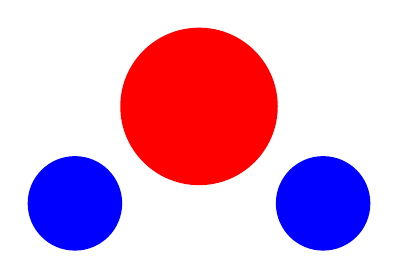
\begin{tikzpicture}[scale=2]
    \fill[red] (0,0) circle (0.5cm);
    \fill[blue] ({-1*sin(52)}, {-1*cos(52)}) circle (0.3cm);
    \fill[blue] ({ 1*sin(52)}, {-1*cos(52)}) circle (0.3cm);
\end{tikzpicture}
\newpage
\noindent
{\large \textbf{Content (fully worked out problems \& answers) continued...}
\\
\begin{tabular}{|p{0.9\linewidth}|}
\hline
\textbf{(6)} A thermometer reads $19.5~^\circ\text{C}$. After heating, it reads $71.5~^\circ\text{C}$.  
What is the temperature change? 
\\ \hline
\end{tabular}
\\
\begin{tabular}{|p{0.9\linewidth}|}
\hline
\textbf{Solution:} $71.5 - 19.5 = 52.0~^\circ\text{C}$ \\
\textit{Plot: Place Hydrogen B at this angle right of vertical, at bond length $r$.} \\
\hline
\end{tabular}
\\
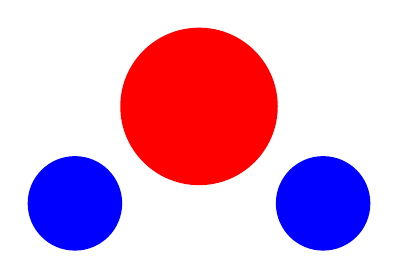
\begin{tikzpicture}[scale=2]
    \fill[red] (0,0) circle (0.5cm);
    \fill[blue] ({-1*sin(52)}, {-1*cos(52)}) circle (0.3cm);
    \fill[blue] ({ 1*sin(52)}, {-1*cos(52)}) circle (0.3cm);
\end{tikzpicture}
\newpage
\noindent
{\large \textbf{Content (fully worked out problems \& answers) continued...}
\\
\begin{tabular}{|p{0.9\linewidth}|}
\hline
\textbf{(7)} An ice cube melts, absorbing $1.00~\text{g}$ of water. Is the sign of $\Delta T$ for the ice positive or negative? 
\\ \hline
\end{tabular}
\\
\begin{tabular}{|p{0.9\linewidth}|}
\hline
\textbf{Solution:} \\
\textit{Plot: Use the sign to confirm that both hydrogens are below oxygen (negative $y$).} \\
\hline
\end{tabular}
\\
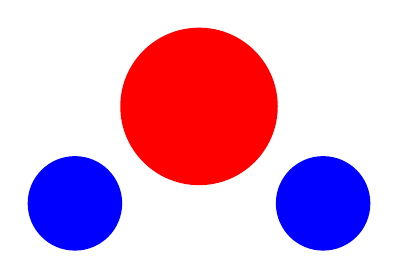
\begin{tikzpicture}[scale=2]
    \fill[red] (0,0) circle (0.5cm);
    \fill[blue] ({-1*sin(52)}, {-1*cos(52)}) circle (0.3cm);
    \fill[blue] ({ 1*sin(52)}, {-1*cos(52)}) circle (0.3cm);
\end{tikzpicture}
\newpage
\noindent
{\large \textbf{Content (fully worked out problems \& answers) continued...}
\\
\begin{tabular}{|p{0.9\linewidth}|}
\hline
\textbf{(8)} Convert $3.0~\text{mm}$ to cm.
\\ \hline
\end{tabular}
\\
\begin{tabular}{|p{0.9\linewidth}|}
\hline
\textbf{Solution:} \\
\textit{Plot: Use this as the radius for each hydrogen nucleus.} \\
\hline
\end{tabular}
\\
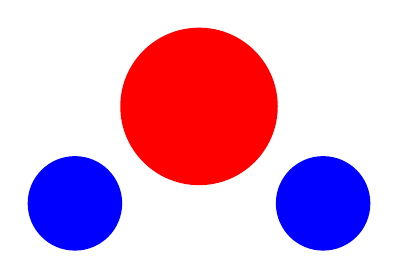
\begin{tikzpicture}[scale=2]
    \fill[red] (0,0) circle (0.5cm);
    \fill[blue] ({-1*sin(52)}, {-1*cos(52)}) circle (0.3cm);
    \fill[blue] ({ 1*sin(52)}, {-1*cos(52)}) circle (0.3cm);
\end{tikzpicture}
\newpage
\noindent
{\large \textbf{Content (fully worked out problems \& answers) continued...}
\\
\begin{tabular}{|p{0.9\linewidth}|}
\hline
\textbf{(9)} Add your two angles from (5) and (6). What total bond angle (with sig figs) do you get?
\\ \hline
\end{tabular}
\\
\begin{tabular}{|p{0.9\linewidth}|}
\hline
\textbf{Solution:} \\
\textit{Plot: Now draw bonds from the oxygen to each hydrogen.} \\
\hline
\end{tabular}
\\
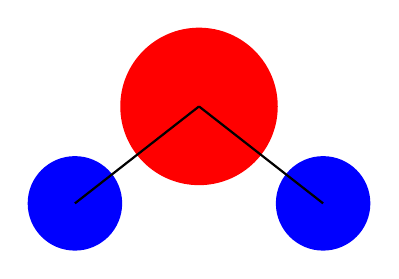
\begin{tikzpicture}[scale=2]
    \fill[red] (0,0) circle (0.5cm);
    \fill[blue] ({-1*sin(52)}, {-1*cos(52)}) circle (0.3cm);
    \fill[blue] ({ 1*sin(52)}, {-1*cos(52)}) circle (0.3cm);
    \draw[thick] (0,0) -- ({-1*sin(52)}, {-1*cos(52)});
    \draw[thick] (0,0) -- ({ 1*sin(52)}, {-1*cos(52)});
\end{tikzpicture}

\newpage


\noindent
{\large \textbf{Checking for Understanding (questions \& answers)}}
\begin{tabular}{|p{0.9\linewidth}|}
\begin{enumerate}
    \item Why is it important to report measurements with the correct number of significant figures? \\
    \textbf{Answer:} To accurately reflect the precision of the measuring instrument and avoid implying more certainty than the measurement supports.
    
    \item When converting $5.0~\text{mm}$ to cm, why do we retain two significant figures? \\
    \textbf{Answer:} Because the original measurement had two significant figures, and unit conversion does not change the precision.

    \item How do positive and negative signs in temperature change or displacement affect plotting? \\
    \textbf{Answer:} Positive values indicate an increase or movement in one direction (up/right), negative values indicate a decrease or movement in the opposite direction (down/left), which determines placement on a coordinate system.

    \item How can multiple measurement results be used to determine a geometric feature like an angle? \\
    \textbf{Answer:} Individual measurements provide numeric values (like temperature change or mass difference) that can be directly mapped to angles or distances, so combining them produces the overall geometry.

    \item Why does plotting measurements in a stepwise manner help build understanding of molecular structure without explicitly naming the molecule? \\
    \textbf{Answer:} It encourages students to see relationships between numbers and positions, reinforcing measurement interpretation and geometric reasoning while keeping the chemical identity hidden.
\end{enumerate} \\
\hline \\
\end{tabular}
\newpage
\noindent
\section*{\underline{Closer}}
\begin{tabular}{|p{4.2cm}|p{9.8cm}|}
\hline
\textbf{Collaborative Learning Techniques} & Personal Favorite \\
\hline
\textbf{Learning Strategy} & Group survey \\
\hline
\textbf{Time} & 12:50---12:55 \\
\hline
\textbf{Materials} & Master periodic table, extra periodic tables \\
\hline
\textbf{Lecture/Textbook/Old Plans/Slide References} & Chapter 2: Measurements \\
\hline
\end{tabular}

\vspace{0.5cm}
\noindent

\noindent
{\large \textbf{Instructions (please provide a \hl{DETAILED} activity breakdown below (and/or attached}}

\begin{tabular}{|p{0.9\linewidth}|}
\hline
\begin{enumerate}[itemsep=0.3em]
    \item Students are given periodic tables to highlight, or highlight on their own periodic table, a chemical element they find interesting.
    \item Highlight a master periodic table to tailor chemical formulas to attending students (don't worry about it if you don't keep track of who highlighted which symbol).
\end{enumerate}
\\ \hline
\end{tabular}

\vspace{0.5cm}
\noindent
{\large \textbf{Content (fully worked out problems \& answers) continued...}

\begin{tabular}{|p{0.9\linewidth}|}
\hline
\begin{itemize}
    \item No new worked problems; personal favorite
\end{itemize}
\\ \hline
\end{tabular}

\vspace{0.5cm}
\noindent
{\large \textbf{Checking for Understanding (questions \& answers)}}

\begin{tabular}{|p{0.9\linewidth}|}
\hline
\begin{itemize}
    \item Review student periodic table favorites
    \item Dedicate time to understanding more about each of their favorites
\end{itemize}
\\ \hline
\end{tabular}
\newpage
\section*{Plan Checklist}

\begin{tabular}{|p{0.9\linewidth}|}
\hline
\begin{itemize}
\item[$\Box$] Variety of Collaborative Learning Techniques and Learning Strategies
\item[$\Box$] Chapter/slide \# where information is coming from
\item[$\Box$] Included timestamps (and buffer time as needed)
\item[$\Box$] Details on how leader will break up students
\item[$\Box$] Checking for Understanding questions
\item[$\Box$] Fully worked out problems and examples for each activity
\item[$\Box$] Necessary links required for online implementation (if applicable)
\item[$\Box$] Source material correctly cited (if applicable)
\item[$\Box$] Plan is uploaded to Teams
\end{itemize}
\\ \hline
\end{tabular}
\newpage

\end{document}
